%!TEX root = ../../../memoria.tex

\section{Productos}

	\subsection{Vista global de productos}\label{chapter:section:productos:subsection:vista_global}
		La interfaz inicial de la aplicación corresponde a la vista de todos los productos que el sistema tiene. En la \refFigura{figure:solution:product:global_view:view} se pueden observar 4 productos.

		\begin{figure}[H]
			\centering
			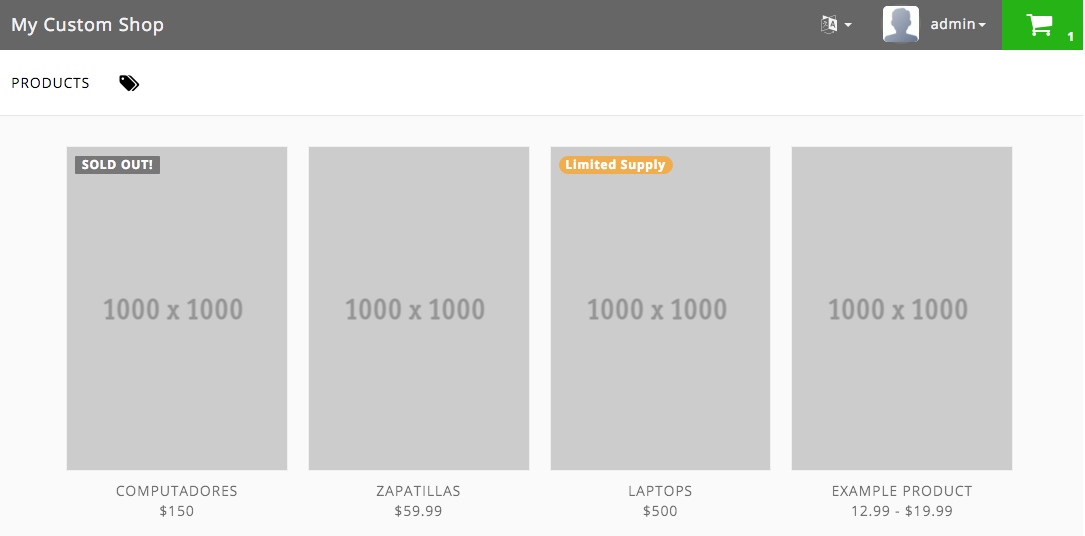
\includegraphics[width=0.8\textwidth]{figuras/solution/product/global_view/view.png}

			\caption{Vista global de los productos. Productos con problemas de \stock dan información.}
			\label{figure:solution:product:global_view:view}
		\end{figure}

		De la interfaz, se observa que hay un producto \textit{SOLD OUT!} y otro producto \textit{LIMITED SUPPLY}. Esto ocurre por que la plataforma tiene un sistema de \trackingCPT de productos la cual puede ser modificada desde la vista \nameref{chapter:section:productos:subsection:edicion}.


		Esta vista depende de los permisos que el usuario que ha ingresado tiene. Si el usuario tiene permisos de edición de productos, tendra la posibilidad de ver todos los productos que existen en el sistema, incluso esos que no estan publicados. En el caso de un usaurio sin permisos de edición, solo tendrá visibilidad de aquellos productos que han sido publicados.

	\subsection{Descripción de un producto}\label{chapter:section:productos:subsection:descripcion}

		La aplicación permite consultar la descripción de un producto. Dicha interfaz puede observarse en la \refFigura{figure:bootstrap:theme_cyborg}. Se puede aprenciar algunas de las carecterísticas de las que ya dispone cada producto.

		\begin{itemize}
			\item
				Un título del producto.
			\item
				Un subtítulo para dar un resumen.
			\item
				Un espacio para la foto del producto.
			\item
				Un lugar para la descripción del producto.
			\item
				Un precio ó intervalo de precios.
		\end{itemize}

	\subsection{Creación de un producto}

		Cuando se penso en la interfaz de creación/edición de un producto, la base era tener una interfaz idéntica a la vista de \nameref{chapter:section:productos:subsection:descripcion}, y por lo tanto, interactuar con los diferentes elementos directamente en la interfaz de vista.
		Cuando se ingresa a la interfaz de vista de un producto con los pemisos adecuados, todas las componenetes de la vista del producto se vuelven componentes editables.

		La interfaz de creación de un producto se observa en la \refFigura{figure:solution:product:create:form}. Es importante destacar la ayuda que brindan los \placeholdersINT para guiar al usuario.

		\begin{figure}[H]
			\centering
			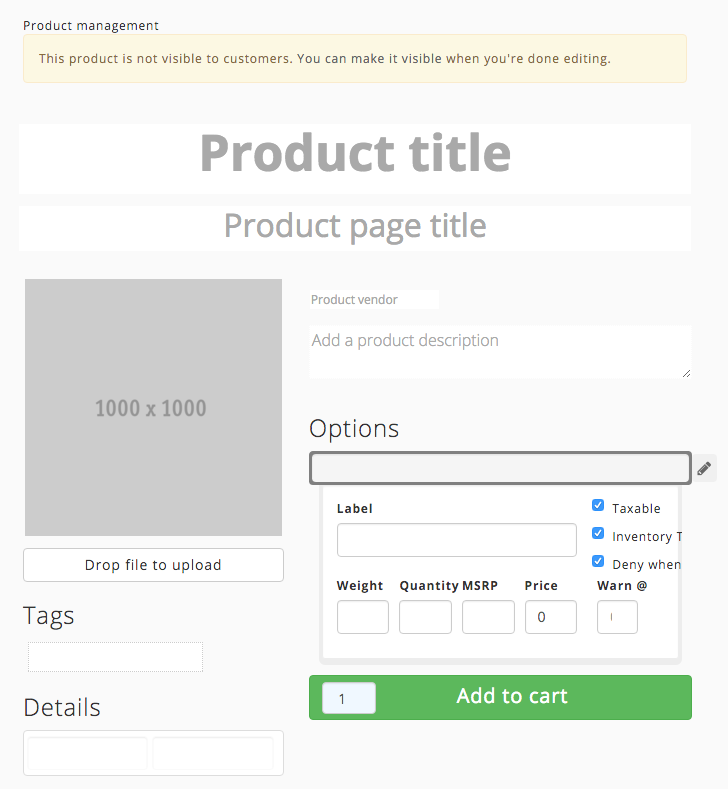
\includegraphics[width=0.8\textwidth]{figuras/solution/product/create/form.png}

			\caption{Interfaz de creación de un producto.}
			\label{figure:solution:product:create:form}
		\end{figure}

		Para determinar los campos utilizados en \refFigura{figure:solution:product:create:form}, de inspiración se utilizó principalmente la interfaz de creación de productos desarollada para el \websiteINT de \shopifyNAME \refFigura{figure:apendice:productos:example:shopify_product_generic_view}. \shopifyNAME es un servicio proporciona toda las herramientas necesarias para desarrollar una tienda \online, razón por la cual cuenta con una gran cantidad de herramientas las cuales no pueden ser avordadas en su totalidad en un contexto de una memoria.
		A continuación se explica cada una de las componenetes utilizadas en el \frameworkPC obtenidas desde  \websiteINT \shopifyNAME:

		\begin{description}
			\item [\titleForm]
				Título principal del producto (\refFigura{figure:product:description:main_tittle}). Idealmente debe ser consiso por que se utiliza tanto en la interfaz de descripción del producto, como en pantalla de búsqueda de productos. El título aparece claramente en la sección principal de la interfaz de creación \refFigura{figure:apendice:productos:example:shopify_product_main}.

				\begin{figure}[H]
					\centering
					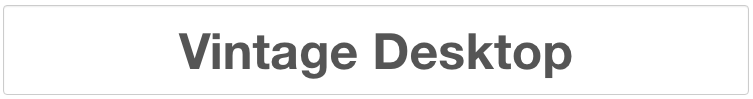
\includegraphics[width=0.6\textwidth]{figuras/product/description/main_tittle.png}

					\caption{Título principal del producto. Aparece también en la lista de búsqueda de productos.}
					\label{figure:product:description:main_tittle}
				\end{figure}

			\item [\pageTitleForm]
				Título exclusivo de la vista \nameref{chapter:section:productos:subsection:descripcion} (\refFigura{figure:product:description:secundary_tittle}). Permite ser más descriptivo que el título. 

				\begin{figure}[H]
					\centering
					\includegraphics[width=0.6\textwidth]{figuras/product/description/secundary_tittle.png}

					\caption{Título secundario del producto. Aparece solo en la página de descripción del producto.}
					\label{figure:product:description:secundary_tittle}
				\end{figure}

			\item [\descriptionForm]
				Permite agregar una descripción del producto(\refFigura{figure:product:description:component_description}). Se encuentra en la sección principal al igual que el \titleForm \refFigura{figure:apendice:productos:example:shopify_product_main}. Esta sección es particularmente importante ( junto con \multimediaForm), por que ayudan en la desición de compra del producto. Es importante agregar descripciones que expliquen el producto, que entreguen \textit{lindas} palabras que fomenten la compra, no una lista de términos técnicos \cite{online_cxpartners_official_people_see_to_buy}.

				\begin{figure}[H]
					\centering
					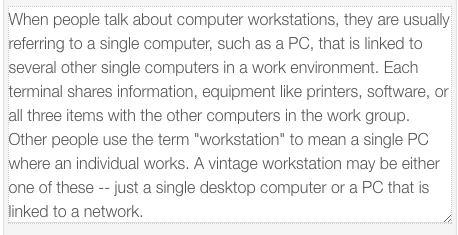
\includegraphics[width=0.6\textwidth]{figuras/product/description/component_description.png}

					\caption{Campo para la descripción del producto.}
					\label{figure:product:description:component_description}
				\end{figure}

			\item [\vendorForm]
				Permite agregar un \vendorForm a la descripción del producto. Aparece en la sección de organización de \shopifyNAME \refFigura{figure:apendice:productos:example:shopify_product_organization}

				\begin{figure}[H]
					\centering
					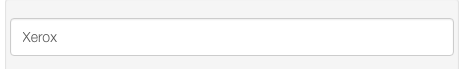
\includegraphics[width=0.6\textwidth]{figuras/product/description/component_vendor.png}

					\caption{Campo para el \vendorForm del producto.}
					\label{figure:product:description:component_vendor}
				\end{figure}

			\item [Options]
				% TODDO : se supone que va aca el \optionsForm
				
			\item [\multimediaForm]
				Al igual como en \shopifyNAME \refFigura{figure:apendice:productos:example:shopify_product_multimedia},esta sección permite agregar imágenes a traves de 2 métodos: \dragdrop y selección utilizando el explorador de archivos \refFigura{figure:product:description:component_multimedia}.
				Las imágenes siempre han sido lo primero que el cliente ve. La mayoria de los \websiteINT ubican las imágenes en la parte superior izquierda de la página \cite{online_cxpartners_official_people_see_to_buy}.
				A diferencia de los compraderos en las tiendas, las imágenes de los productos son la única forma real de determinar si un producto se ajusta a sus necesidades y a sus preferencias. Es una manera poderosa de darle vitrina a los productos. Por lo tanto es muy importante proveer de imágenes de buena calidad entre otros detalles \cite{online_cxpartners_official_people_see_to_buy}. Esto explica el tamaño de imagen que se acepta en la plataforma.

				\begin{figure}[H]
					\centering
					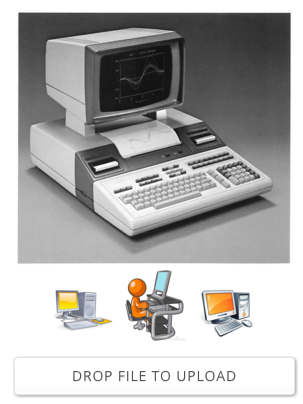
\includegraphics[width=0.6\textwidth]{figuras/product/description/component_multimedia.png}

					\caption{Sección de las imágenes del producto.}
					\label{figure:product:description:component_multimedia}
				\end{figure}
				
			\item [\tagsForm]
				Provenientes de la sección organización \refFigura{figure:apendice:productos:example:shopify_product_organization}, permite la categorización utilisando palabras clave relevantes.

				\begin{figure}[H]
					\centering
					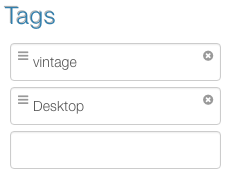
\includegraphics[width=0.6\textwidth]{figuras/product/description/component_tags.png}

					\caption{Campo para las \tagsForm del producto.}
					\label{figure:product:description:component_tags}
				\end{figure}
				
		\end{description}

		También se tuvo en consideración la siguiente información al momento de desarrollar esta interfaz:

		\begin{itemize}
			\item Los visitantes prefieren imágenes de los productos a la izquierda y la descripción a la derecha \cite{online_cxpartners_official_people_see_to_buy}.
			\item Es improbable que un usuario haga \scrollCPT(en el caso de interfaces \desktop) para ver más contenido en la página \cite{online_cxpartners_official_people_see_to_buy}.
			\item Usuarios nunca o muy rara vez leen toda la información disponible especialmente cuando hay muchísimo contenido. Usualmente se ignora la parte inferior o recorren sin poner atención a todas las secciones. E incluso si hacen \scrollCPT, ellos no necesariamente leen o ponen atención a todo el contenido inferior de la página \cite{online_cxpartners_official_people_see_to_buy}.
			%Customers never, or hardly ever read everything you put on the page especially when there is a lot of content! Even if it has a good layout, a long page does not work well. Users often ignore the bottom bits or skim through without paying attention to all sections. And even if they do scroll down, they do not necessarily read or pay attention to all the content below the page.
			\item Agregar solo la información importante del producto que se venderá \cite{online_cxpartners_official_people_see_to_buy}.

			\item Proveer un espació razonable y no sobre utilizar colores \cite{online_cxpartners_official_people_see_to_buy}.

			\item Evitar el uso de \clicking si se desea que el usuario lea \cite{online_cxpartners_official_people_see_to_buy}.
		\end{itemize}


		De los campos que se observan en la \refFigura{figure:solution:product:create:form}: \titleForm, \pageTitleForm, \vendorForm, \descriptionForm, \tagsForm y \detailsForm, tienen \feedbackReactivoDEF. Las restricciones en la creación de un producto se encuentra en la \reftabla{tab:solution:products:create:form:product:generic}. 

		\begin{table}[H]
		    \centering
			\begin{tabular}{ |l|c||l| }
				\hline Campo & Requerido & Restricción \\ \hline
				\multirow{1}{*}{\titleForm} 			&  \multirow{1}{*}{\checkmark} & - Debe tener al menos un caracter. \\ \hline
				\multirow{1}{*}{\pageTitleForm} 	&  \multirow{1}{*}{} &  \\ \hline
				\multirow{1}{*}{\vendorForm}		&  \multirow{1}{*}{} &  \\ \hline
				\multirow{1}{*}{\optionsForm}		&  \multirow{1}{*}{\checkmark} &  \\ \hline
				\multirow{1}{*}{\descriptionForm}	&  \multirow{1}{*}{} &  \\ \hline
				\multirow{1}{*}{\multimediaForm}	&  \multirow{1}{*}{} &  \\ \hline
				\multirow{1}{*}{\tagsForm}			&  \multirow{1}{*}{} &  \\ \hline
				%\multirow{1}{*}{\detailsForm}		&  \multirow{1}{*}{} &  \\ \hline
			\end{tabular}
		 	\caption{Resumen restrincciones para formulario creación de un producto.}
		    \label{tab:solution:products:create:form:product:generic}
		\end{table}

		Como se aprecia en la \reftabla{tab:solution:products:create:form:product:generic}, el campo \detailsForm no es requerido, sin embargo, cada \detailForm en realidad es un objeto compuesto cuyos campos si son obligatorios(\reftabla{tab:solution:products:create:form:product:generic:details}).

		\begin{table}[H]
		    \centering
			\begin{tabular}{ |l|c||l| }
				\hline Campo & Requerido & Restricción \\ \hline
				\multirow{1}{*}{\textit{Anónimo key}}	&  \multirow{1}{*}{\checkmark} & - Debe tener al menos un caracter. \\ \hline
				\multirow{1}{*}{\textit{Anónimo Value}}	&  \multirow{1}{*}{\checkmark} & - Debe tener al menos un caracter. \\ \hline
			\end{tabular}
		 	\caption{Resumen restrincciones para formulario creación de \detailsForm.}
		    \label{tab:solution:products:create:form:product:generic:details}
		\end{table}

		Si no enfocamos en los campos de la \refFigura{figure:product:description:product_options} se observa que ellos se encuentran repartidos entre las secciones \PricingForm(\refFigura{figure:apendice:productos:example:shopify_product_princing}), \InventoryForm(\refFigura{figure:apendice:productos:example:shopify_product_inventory}), \ShippingForm(\refFigura{figure:apendice:productos:example:shopify_product_shipping}) y \VariantsForm(\refFigura{figure:apendice:productos:example:shopify_product_variant_max}).

		\begin{description}
			\item [\LabelForm]
				Corresponde al nombre de la \VariantsForm del producto que se utiliza.

			\item [\OptionForm]
				Se utiliza para identificar cada una de las \VariantsForm al momento de agregarlas al carro.

			\item [\WeightForm]
				Corresponde al peso (masa), del producto que se esta ofreciendo. Este valor se utiliza para \shipping, razón por la cual aparece esta componente en la sección \ShippingForm del formulario de \shopifyNAME \refFigura{figure:apendice:productos:example:shopify_product_shipping}.

			\item [\trackingForm]
				Permite tomar acciones dependiendo del inventario que se tenga. Ver \refFigura{figure:apendice:productos:example:shopify_product_inventory}.

			\item [\denyForm]
				Al igual que el la sección \InventoryForm de \shopifyNAME(\refFigura{figure:apendice:productos:example:shopify_product_inventory}), esta componente aparece cuando se ha seleccionado la opción de \trackingForm. Esta opción evita que los clientes sigan comprando el producto una vez que se ha terminado el inventario.

			\item [\taxableForm]
				Aplica Cargos de impuesto al producto.

			\item [\quantityForm]
				Cantidad de elementos para este producto en particular.

			\item [\priceForm]
				Precio de este producto en particular.
		\end{description}

		\begin{figure}[H]
			\centering
			\includegraphics[width=0.6\textwidth]{figuras/product/description/product_options.png}

			\caption{Sección de las opciones del producto.}
			\label{figure:product:description:product_options}
		\end{figure}

		\begin{table}[H] 
		    \centering
			\begin{tabular}{ |l|c||l| }
				\hline Campo & Requerido & Restricción \\ \hline
				\multirow{1}{*}{\textit{Label}}		&  \multirow{1}{*}{\checkmark} 	& - Debe tener al menos un caracter \\ \hline
				\multirow{1}{*}{\textit{\WeightForm}}	&  \multirow{1}{*}{\checkmark} 	& - Número racional mayor o igual a '0' \\ \hline
				\multirow{1}{*}{\quantityForm}	&  \multirow{1}{*}{\checkmark} 	& - Número entero \\ \hline
				\multirow{1}{*}{\msrpSIGLAS}		&  \multirow{1}{*}{} 			& - Número racional mayor o igual a '0' \\ \hline
				\multirow{1}{*}{\priceForm}		&  \multirow{1}{*}{\checkmark} 	& - Número racional mayor o igual a '0' \\ \hline
				\multirow{1}{*}{\denyForm}		&  \multirow{1}{*}{\checkmark} 	& - Boolean \\ \hline
				\multirow{1}{*}{\warnForm}		&  \multirow{1}{*}{} 			& - Número racional mayor o igual a '0' \\ \hline
				\multirow{1}{*}{\taxableForm}	&  \multirow{1}{*}{\checkmark} 	& - Boolean \\ \hline
				\multirow{1}{*}{\trackingForm}	&  \multirow{1}{*}{\checkmark} 	& - Boolean \\ \hline
			\end{tabular}
		 	\caption{Resumen restrincciones para formulario creación de \optionsForm.}
		    \label{tab:solution:products:create:form:product:generic:options}
		\end{table}

	\subsection{Edición de un producto}\label{chapter:section:productos:subsection:edicion}

		Al igual que para la creación de productos, la edición requiere de permisos especiales. Si se cuenta con dichos permisos especiales, la interfaz de la vista de un producto inmediatamente permite editar los campos. Para editarlos, simplemente es necesario seleccionar la componente con el \mousePC y hacer un \click. La componente cambiara su aspecto para dar \feedback al usuario de que esta seleccionada dicha componente y que puede realizar sobre el ediciones. En la \refFigura{figure:features:interfaz_edicion_editando_description} y \ref{figure:features:interfaz_edicion_editando_subtitulo} es posible apreciar la componentes que se ha seleccionado para editar.

		\begin{figure}[H]
			\centering
			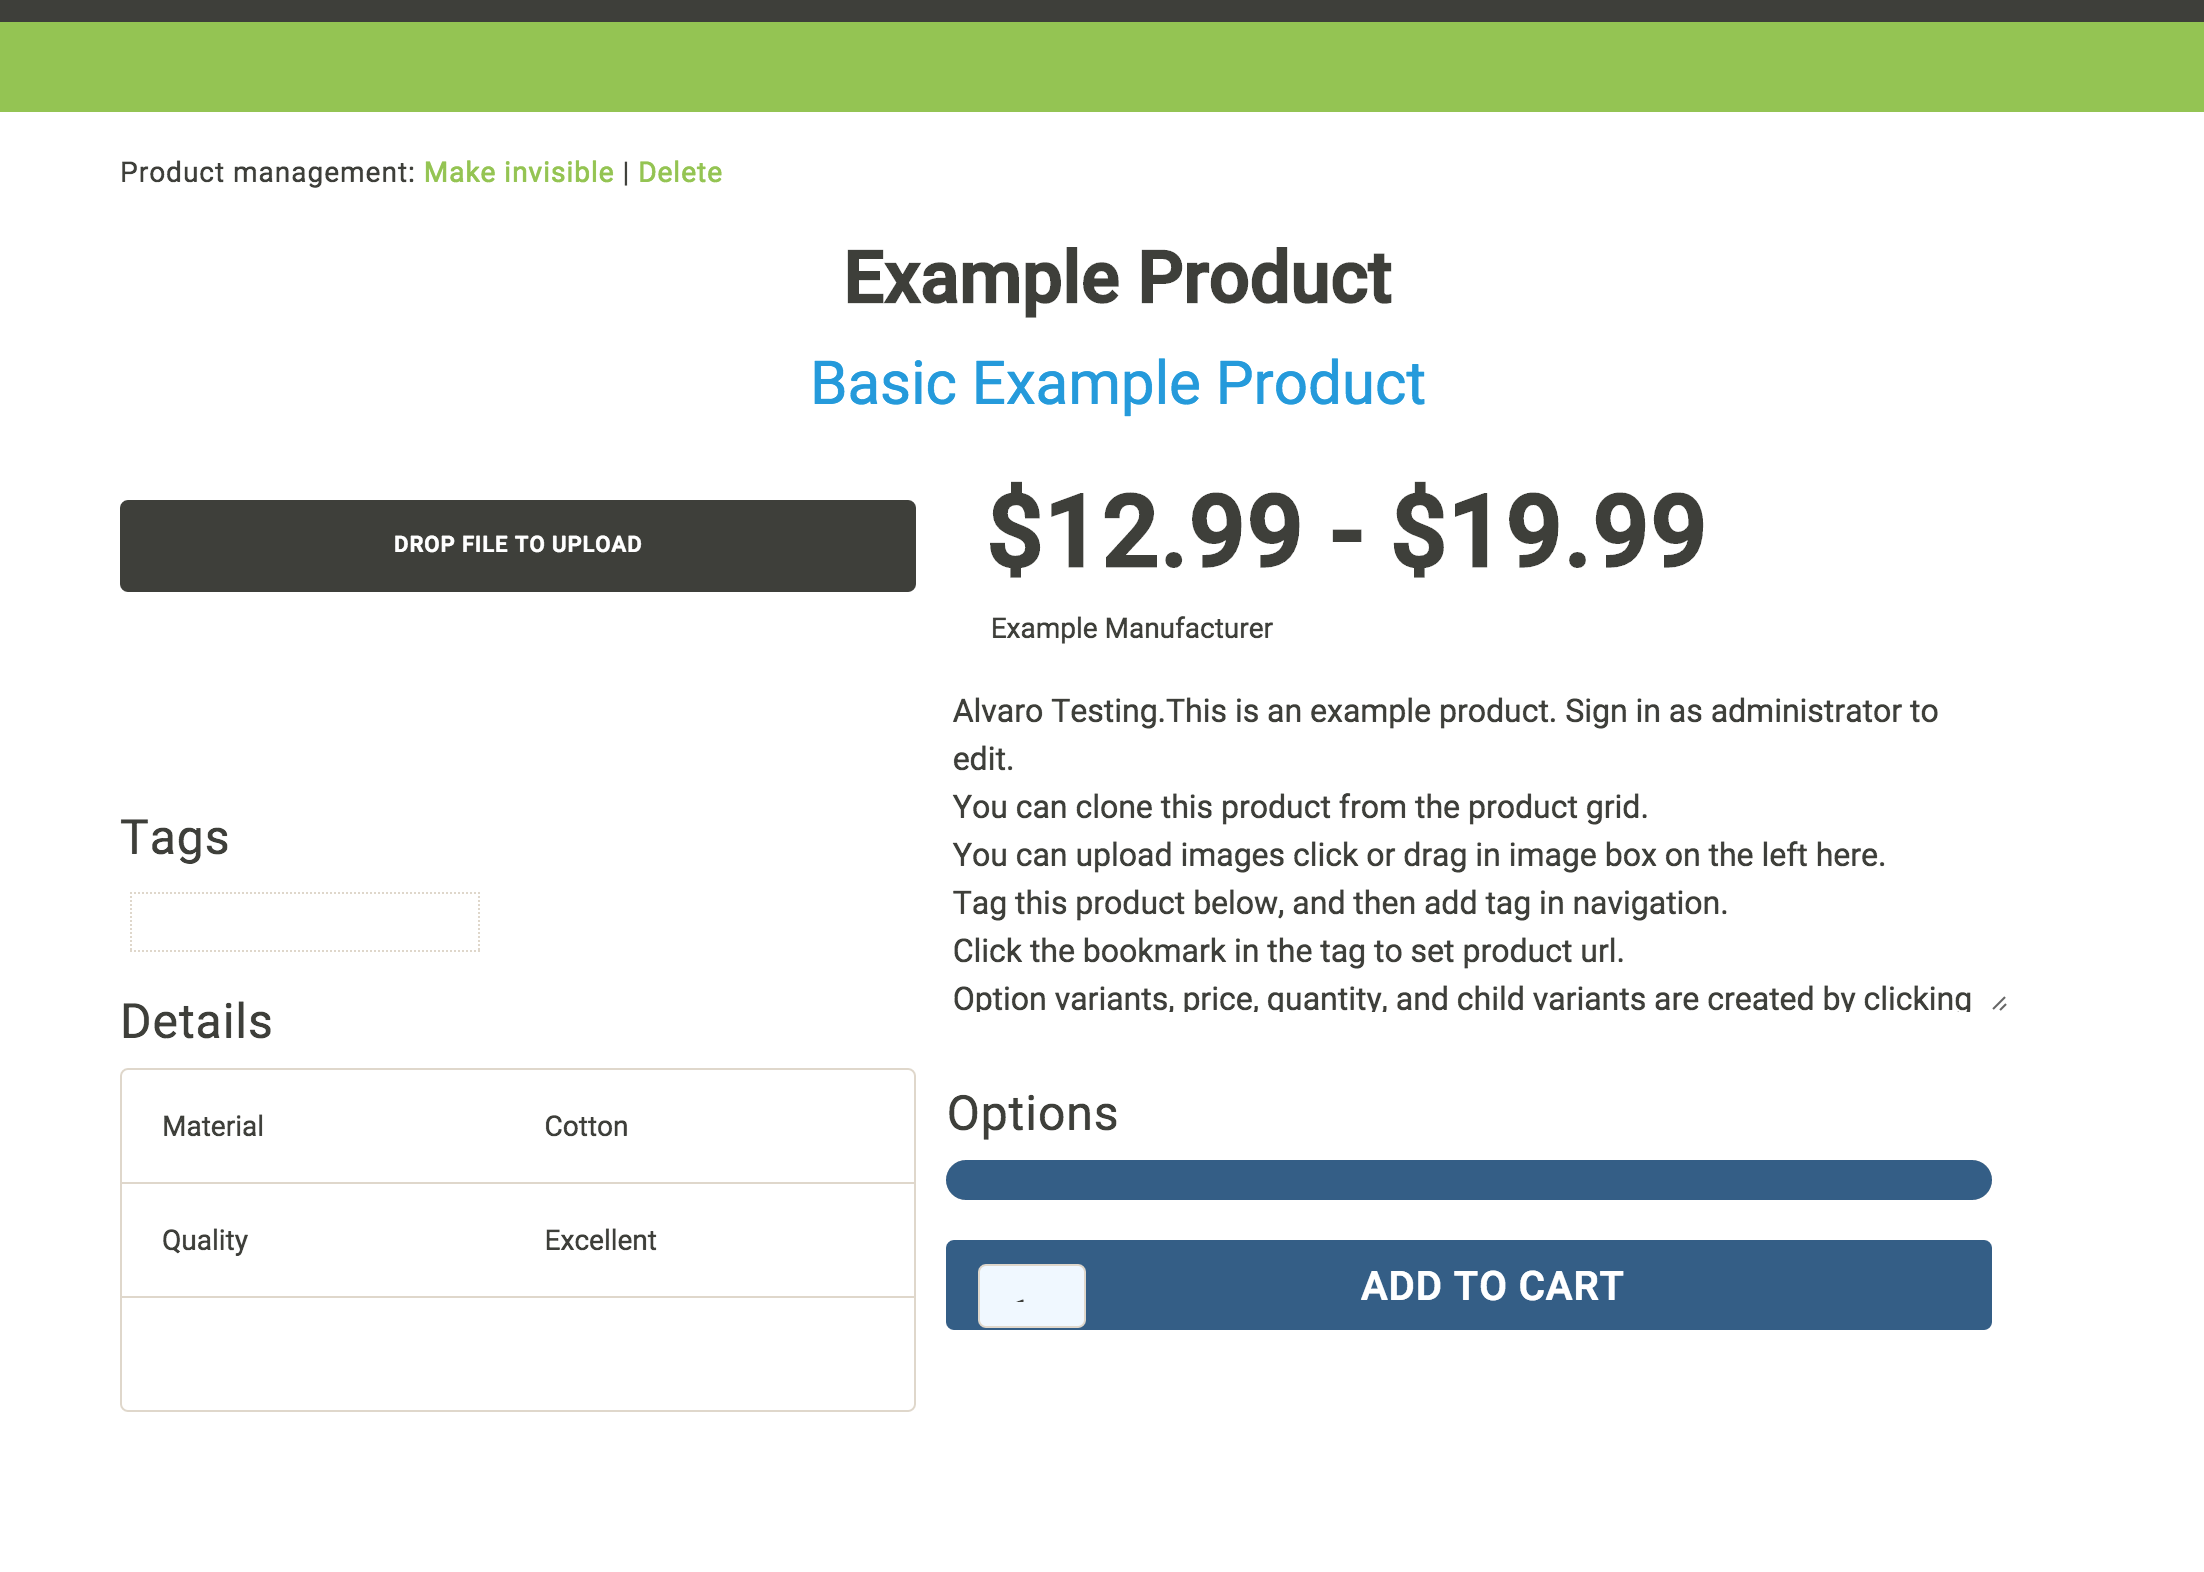
\includegraphics[width=0.8\textwidth]{figuras/productos/interfaz_edicion_producto.png}

			\caption{Interfaz de la edición de un producto.}
			\label{figure:features:interfaz_edicion_producto}
		\end{figure}

		\begin{figure}[H]
			\centering
			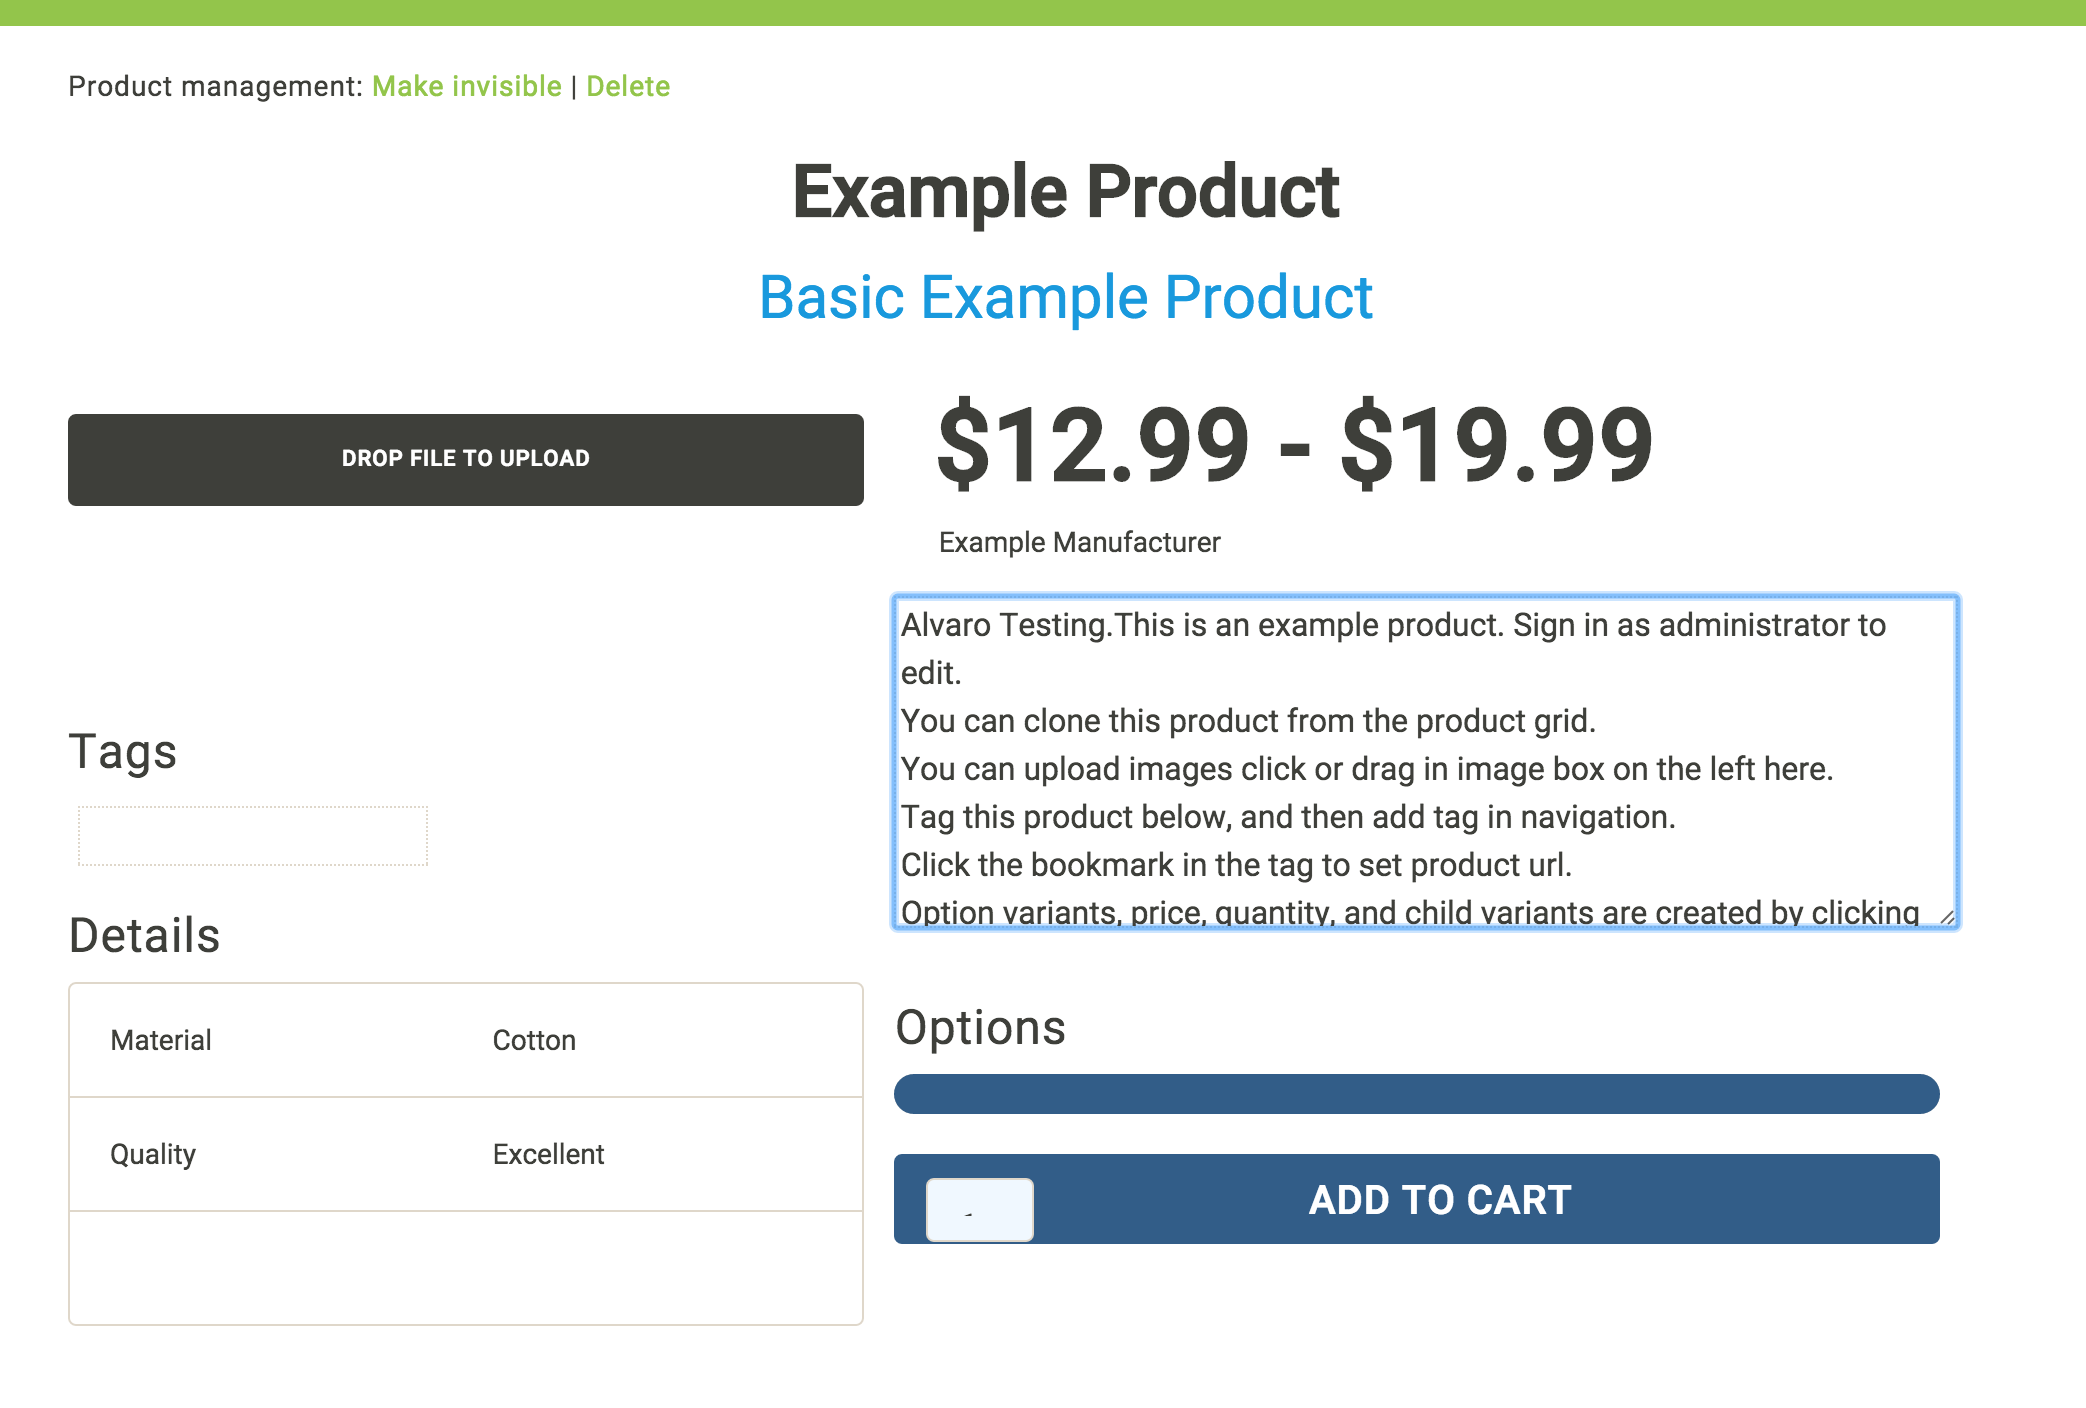
\includegraphics[width=0.8\textwidth]{figuras/productos/interfaz_edicion_editando_description.png}

			\caption{Campo descripción seleccionado para edición.}
			\label{figure:features:interfaz_edicion_editando_description}
		\end{figure}


		\begin{figure}[H]
			\centering
			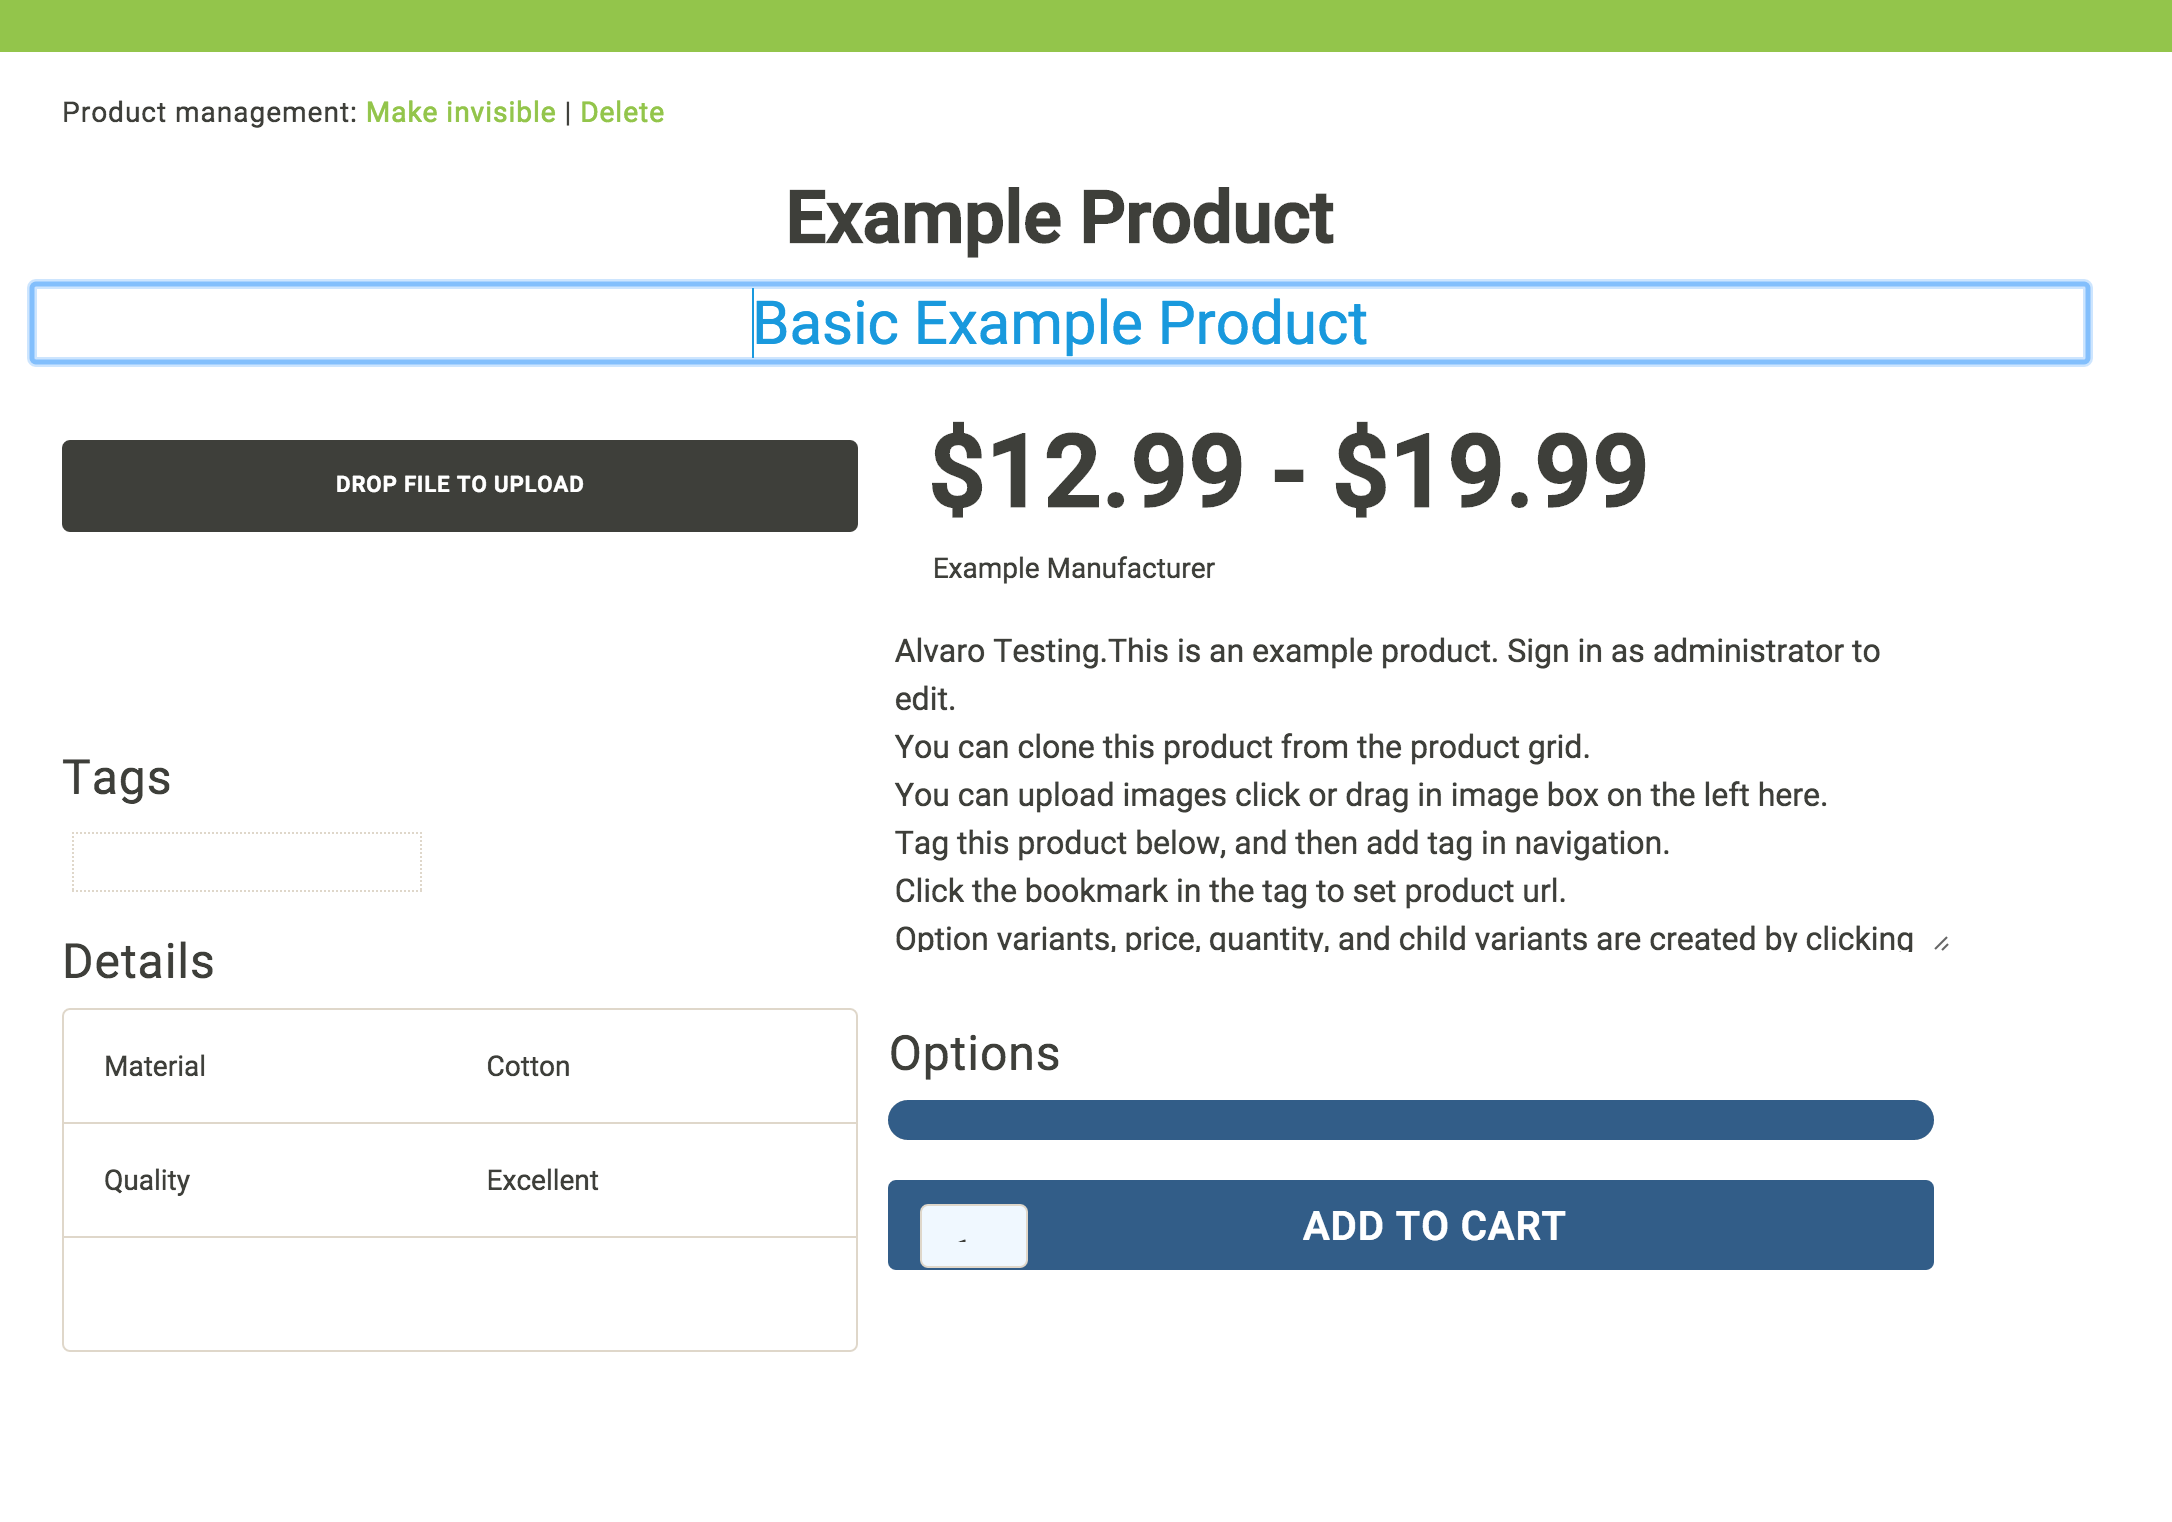
\includegraphics[width=0.8\textwidth]{figuras/productos/interfaz_edicion_editando_subtitulo.png}

			\caption{Campo subtítulo seleccionado para edición.}
			\label{figure:features:interfaz_edicion_editando_subtitulo}
		\end{figure}

		Es importante mencionar que la edición de producto es \reactive, por lo tanto todos los cambios que se realizen serán inmediatamente visibles por parte de todos los usuarios que esten mirando la descripción del producto incluso sin la necesidad de que el usuario haga un \refreshCPT del \websiteINT.

	%TODO: Agregar esta seccion en el futuro
	%\subsection{Eliminación de un producto}

	\subsection{Visibilidad de un producto}
	
		Todo producto válido puede ser visible para todos los usuarios(visibilidad global), o solo visible para aquellos que tienen permiso de edición sobre dicho producto. Esta importante característica se encuentra disponible en el servicio de \shopifyNAME(\refFigura{figure:apendice:productos:example:shopify_product_visibility}). En la \refFigura{figure:solution:product:visibility:new} se ve el caso particular de un producto que esta en proceso de creación (no tiene título, el cual es requerido).

		\begin{figure}[H]
			\centering
			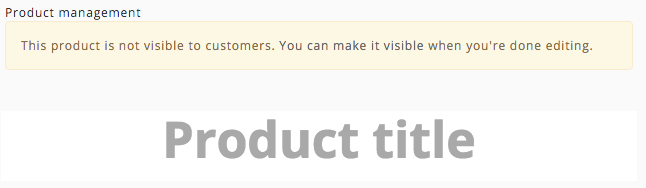
\includegraphics[width=0.8\textwidth]{figuras/solution/product/visibility/new.png}

			\caption{Producto con visibilidad limitada. Notar que no tiene título, lo que implíca que no es un producto válido aún.}
			\label{figure:solution:product:visibility:new}
		\end{figure}

		Después de llenar todos los campos mínimos requeridos para la creación de un producto, es posible presionar el \linkINT \youCanMakeItVisibleLABEL y dar visibilidad global al producto. En el caso que no estén llenos todos los campos requerídos, entonces se generá un \autoFocoINT del primer campo no completado requerido. Suponiendo que se intenta dar visibilidad del producto de la \refFigura{figure:solution:product:visibility:new}, se hara un \autoFocoINT del campo título, el cual puede observarse en la \refFigura{figure:solution:product:visibility:autofocus}; además de mantener el estado de visibilidad (no visible para todos). Esto ocurre para mostrar claramente al usuario que esta sucediendo \cite{online_google_ui_pattern_error,online_goodgui_org}.

		\begin{figure}[H]
			\centering
			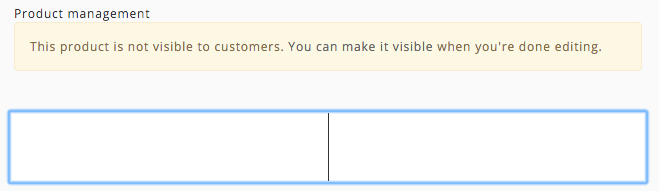
\includegraphics[width=0.8\textwidth]{figuras/solution/product/visibility/autofocus.png}

			\caption{Resultado tras dar visibilidad a un producto sin título. Se genera un \autoFocoINT en el campo título, dado que este es requerido y el estado de visibilidad del producto continua igual.}
			\label{figure:solution:product:visibility:autofocus}
		\end{figure}

		Si todos los campos requeridos de un producto están completos, y se presiona el \linkINT \youCanMakeItVisibleLABEL, se tendra el resultado de la \refFigura{figure:solution:product:visibility:global_visibility}; en donde se observa como el texto superior cambío. Ahora aparece un \linkINT con el texto \makeInvisibleLABEL, para dar \feedback al usuario de lo que ha ocurrido \cite{online_google_ui_design_material,online_goodgui_org}.

		\begin{figure}[H]
			\centering
			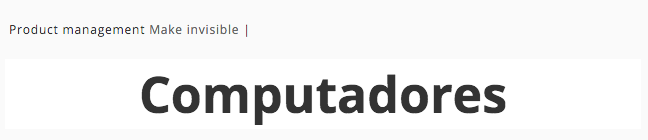
\includegraphics[width=0.8\textwidth]{figuras/solution/product/visibility/global_visibility.png}

			\caption{Producto con visibilidad global. Aparece un \linkINT \makeInvisibleLABEL para ocultar el producto.}
			\label{figure:solution:product:visibility:global_visibility}
		\end{figure}

		%Si se intenta dar visibilidad global de un producto que no esta completo (ver requerimientos de \reftabla{tab:solution:products:create:form:product:generic}), se hará un autofoco al primer elmemento que sea requerido pero que no este completo. Como ejemplo, vemos la \refFigura{figure:solution:product:visibility:new} 	
